
\subsubsection{Analisi Derivazioni e Ridondanze}

\paragraph[H]{Attributo Difesa}L'unico dato derivabile che viene utilizzato dalle nostre operazione  la Difesa del Personaggio (operazioni 13,14,19,20,46). L'attributo in questione pu\`{o} essere ricavato dalla somma della difesa degli oggetti indossati e dalla somma della difesa delle occorrenze dell'entit\`{a} consumo. Di seguito si valuta la convenienza di utilizzo del dato difesa.



\begin{table}[H]
\centering
\caption{Operazione 13}
\begin{tabular}{llll}
\\ \hline
\multicolumn{1}{|l|}{\textbf{CONCETTO}} & \multicolumn{1}{l|}{\textbf{COSTRUTTO}} & \multicolumn{1}{l|}{\textbf{ACCESSI}} & \multicolumn{1}{l|}{\textbf{TIPO}} \\ \hline
\multicolumn{1}{|l|}{Indossamento}      & \multicolumn{1}{l|}{R}                  & \multicolumn{1}{l|}{1}                & \multicolumn{1}{l|}{L}             \\ \hline
\multicolumn{1}{|l|}{Stock}             & \multicolumn{1}{l|}{R}                  & \multicolumn{1}{l|}{1}                & \multicolumn{1}{l|}{L}             \\ \hline
\multicolumn{1}{|l|}{Indossamento}      & \multicolumn{1}{l|}{R}                  & \multicolumn{1}{l|}{2}                & \multicolumn{1}{l|}{S}             \\ \hline
\multicolumn{1}{|l|}{Stock}             & \multicolumn{1}{l|}{R}                  & \multicolumn{1}{l|}{2}                & \multicolumn{1}{l|}{S}             \\ \hline
\end{tabular}
\end{table}


\begin{table}[H]
\centering
\caption{Operazione 14}
\label{my-label}
\begin{tabular}{|l|l|l|l|}
\hline
\textbf{CONCETTO} & \textbf{COSTRUTTO} & \textbf{ACCESSI} & \textbf{TIPO} \\ \hline
Consumo           & E                  & 1                & S             \\ \hline
Consumante        & R                  & 1                & S             \\ \hline
Consunto          & R                  & 1                & S             \\ \hline
\end{tabular}
\end{table}


\begin{table}[H]
\centering
\caption{Operazione 19}
\label{my-label}
\begin{tabular}{|l|l|l|l|}
\hline
\textbf{CONCETTO} & \textbf{COSTRUTTO} & \textbf{ACCESSI} & \textbf{TIPO} \\ \hline
Personaggio       & E                  & 1                & L             \\ \hline
Equipaggiamento   & E                  & 1                & L             \\ \hline
Indossamento      & R                  & 1                & S             \\ \hline
\end{tabular}
\end{table}

\begin{table}[H]
\centering
\caption{Operazione 20}
\label{my-label}
\begin{tabular}{|l|l|l|l|}
\hline
\textbf{CONCETTO} & \textbf{COSTRUTTO} & \textbf{ACCESSI} & \textbf{TIPO} \\ \hline
Consumo           & E                  & 1                & L             \\ \hline
Consumo           & E                  & 1                & S             \\ \hline
\end{tabular}
\end{table}


\begin{table}[H]
\centering
\caption{Operazione 46}
\label{my-label}
\begin{tabular}{|l|l|l|l|}
\hline
\textbf{CONCETTO} & \textbf{COSTRUTTO} & \textbf{ACCESSI} & \textbf{TIPO} \\ \hline
Consunto          & R                  & 1                & L             \\ \hline
Consumabili       & E                  & 1                & L             \\ \hline
Consumo           & E                  & 1                & L             \\ \hline
\end{tabular}
\end{table}




\begin{table}[H]
\centering
\caption{Operazione 13}
\label{my-label}
\begin{tabular}{|l|l|l|l|}
\hline
\textbf{CONCETTO} & \textbf{COSTRUTTO} & \textbf{ACCESSI} & \textbf{TIPO} \\ \hline
Indossamento      & R                  & 1                & L             \\ \hline
Stock             & R                  & 1                & L             \\ \hline
Indossamento      & R                  & 2                & S             \\ \hline
Stock             & R                  & 2                & S             \\ \hline
Personaggio       & E                  & 1                & L             \\ \hline
Personaggio       & E                  & 1                & L             \\ \hline
\end{tabular}
\end{table}



\begin{table}[H]
\centering
\caption{Operazione 14}
\label{my-label}
\begin{tabular}{|l|l|l|l|}
\hline
\textbf{CONCETTO} & \textbf{COSTRUTTO} & \textbf{ACCESSI} & \textbf{TIPO} \\ \hline
Consumo           & E                  & 1                & S             \\ \hline
Consumante        & R                  & 1                & S             \\ \hline
Consunto          & R                  & 1                & S             \\ \hline
Personaggio       & E                  & 1                & L             \\ \hline
Personaggio       & E                  & 1                & L             \\ \hline
\end{tabular}
\end{table}


\begin{table}[H]
\centering
\caption{Operazione 19}
\label{my-label}
\begin{tabular}{|l|l|l|l|}
\hline
\textbf{CONCETTO} & \textbf{COSTRUTTO} & \textbf{ACCESSI} & \textbf{TIPO} \\ \hline
Personaggio       & E                  & 1                & L             \\ \hline
Equipaggiamento   & E                  & 1                & L             \\ \hline
Indossamento      & R                  & 1                & S             \\ \hline
Personaggio       & E                  & 1                & L             \\ \hline
Personaggio       & E                  & 1                & L             \\ \hline
\end{tabular}
\end{table}


\begin{table}[H]
\centering
\caption{Operazione 20}
\label{my-label}
\begin{tabular}{|l|l|l|l|}
\hline
\textbf{CONCETTO} & \textbf{COSTRUTTO} & \textbf{ACCESSI} & \textbf{TIPO} \\ \hline
Consumo           & E                  & 1                & L             \\ \hline
Consumo           & E                  & 1                & S             \\ \hline
Personaggio       & E                  & 1                & L             \\ \hline
Personaggio       & E                  & 1                & L             \\ \hline
\end{tabular}
\end{table}

\begin{table}[H]
\centering
\caption{Operazione 46}
\label{my-label}
\begin{tabular}{|l|l|l|l|}
\hline
\textbf{CONCETTO} & \textbf{COSTRUTTO} & \textbf{ACCESSI} & \textbf{TIPO} \\ \hline
Consunto          & R                  & 1                & L             \\ \hline
Consumabili       & E                  & 1                & L             \\ \hline
Consumo           & E                  & 1                & L             \\ \hline
Personaggio       & E                  & 1                & L             \\ \hline
Personaggio       & E                  & 1                & L             \\ \hline
\end{tabular}
\end{table}




\begin{table}[H]
\centering
\caption{Costo Operazioni senza ridondanza}
\label{my-label}
\resizebox{\textwidth}{!}{%
\begin{tabular}{|l|l|l|l|}
\hline
\textbf{OPERAZIONE}               & \textbf{COSTO} & \textbf{FREQUENZA} & \textbf{TOTALE} \\ \hline
13                                & 10             & 100000             & 1000000         \\ \hline
14                                & 6              & 87500              & 525000          \\ \hline
19                                & 4              & 100000             & 400000          \\ \hline
20                                & 3              & 87500              & 262500          \\ \hline
46                                & 3              & 100000             & 300000          \\ \hline
COSTO OPERAZIONI SENZA RIDONDANZA & \hl{2487500}        &                    &                 \\ \hline
\end{tabular}
}
\end{table}

\begin{table}[H]
\centering
\caption{Costo Operazioni con Ridondanza}
\label{my-label}
\resizebox{\textwidth}{!}{%
\begin{tabular}{|l|l|l|l|}
\hline
\textbf{OPERAZIONE}             & \textbf{COSTO} & \textbf{FREQUENZA} & \textbf{TOTALE} \\ \hline
13                              & 13             & 100000             & 1300000         \\ \hline
14                              & 9              & 87500              & 787500          \\ \hline
19                              & 7              & 100000             & 700000          \\ \hline
20                              & 6              & 87500              & 525000          \\ \hline
46                              & 6              & 100000             & 600000          \\ \hline
COSTO OPERAZIONI CON RIDONDANZA & \hl{3912500}        &                    &                 \\ \hline
\end{tabular}
}
\end{table}

Alla luce della di quanto visto precedentemente abbiamo riscontrato un aumento del costo delle operazioni con la Ridondanza di circa il 40\%, si rende quindi necessario eliminare tale Dato.


\newpage
\subsubsection{Eliminazione Delle Gerarchie}

Nel nostro schema concettuale sono presenti 5 generalizzazioni. Le Entità coinvolte sono "PA, Azienda o Persona", "Cliente", "Richiesta sul Mepa", "Prodotto o servizio", "Prodotto".
\newline
Abbiamo deciso di procedere nel seguente modo:

\paragraph{PA, Azienda o Persona}
Per quanto riguarda l'entità PA, Azienda o Persona, abbiamo scelto di accorpare il genitore della generalizzazione nelle entità figlie. Questo perchè i clienti e i fornitori hanno rapporti con l'azienda piuttosto diversi tra loro, quindi la separazione comporta una suddivisione concettuale che migliora la chiarezza dello schema.
\paragraph{Cliente}
Per l'entità Cliente si è optato di mantenere il genitore e mantenere le entità figlie, in quanto un eventuale accorpamento del genitore nelle entità figlie complicherebbe lo schema, viste le numerose relazioni che ha il genitore. Abbiamo sostituito la generalizzazione con delle relazioni, denominate "Specificazione Privato" e "Specificazione PA".
\paragraph{Richiesta sul Mepa}
In merito all'entità Richiesta sul Mepa, si è scelto l'accorpamento del genitore della generalizzazione nelle entità figlie. Si avrebbe potuto accorpare le entità figlie nel genitore, utilizzando degli attributi che possono assumere il valore NULL per poter distinguire appunto le due entità, ma ci sembra più opportuno mantenere distinte le entità Gara pubblica e Trattativa diretta in quanto esse sono, nella realtà pratica, due concetti logicamente separati. Il mantenimento della loro suddivisione permette quindi una maggior comprensibilità dello schema.
\paragraph{Prodotto o Servizio}
Per quanto riguarda l'entità Prodotto o Servizio, abbiamo deciso di mantenere le entità figlie ed eliminare il genitore, in quanto ogni operazione che coinvolge il padre comprende almeno uno dei figli.
\paragraph{Prodotto}
Per l'entità Prodotto si è scelto di mantenere sia il padre che le entità figlie, dato che queste ultime hanno tanti attributi diversi, e l'accorpamento nell'entità genitore significherebbe avere tanti valori con valore NULL. Inoltre, un eventuale accorpamento del genitore nelle entità figlie risulterebbe piuttosto complicato, date le numerose relazioni che ha il padre e visto che le entità figlie sono molteplici.
Quindi, si è scelto di sostituire la generalizzazione con delle relazioni, una per ogni entità figlia. Le nuove relazioni sono denominate "Specificazione" più il nome dell'entità a cui si riferiscono.
\newline\newline
In seguito all'eliminazione delle generalizzazioni di Cliente e Prodotto, è necessario imporre delle nuove regole di vincolo, per evitare errori logici:

\begin{itemize}
  \item Ogni occorrenza di "Cliente" deve essere occorrenza o di "Privato" o di "Pubblica Amministrazione". Non potrà essere occorrenza contemporaneamente di entrambe queste entità.
  \item Ogni occorrenza di "Prodotto" deve essere occorrenza o di "Notebook" o di "Pc Desktop" o di "Monitor" o di "Stampante". Non potrà essere occorrenza contemporaneamente di due o più di queste entità.
\end{itemize}
\noindent
\textit{(Facciamo notare che, per non appesantire ulteriormente lo schema, abbiamo scelto di togliere alcuni prodotti e di mantenere solo "Notebook", "Pc Desktop", "Monitor", "Stampante".)}




% \newpage
%
%
% \begin{landscape} %inizia un foglio landscape
%
% %include un file pdf che contiene lo schema
% 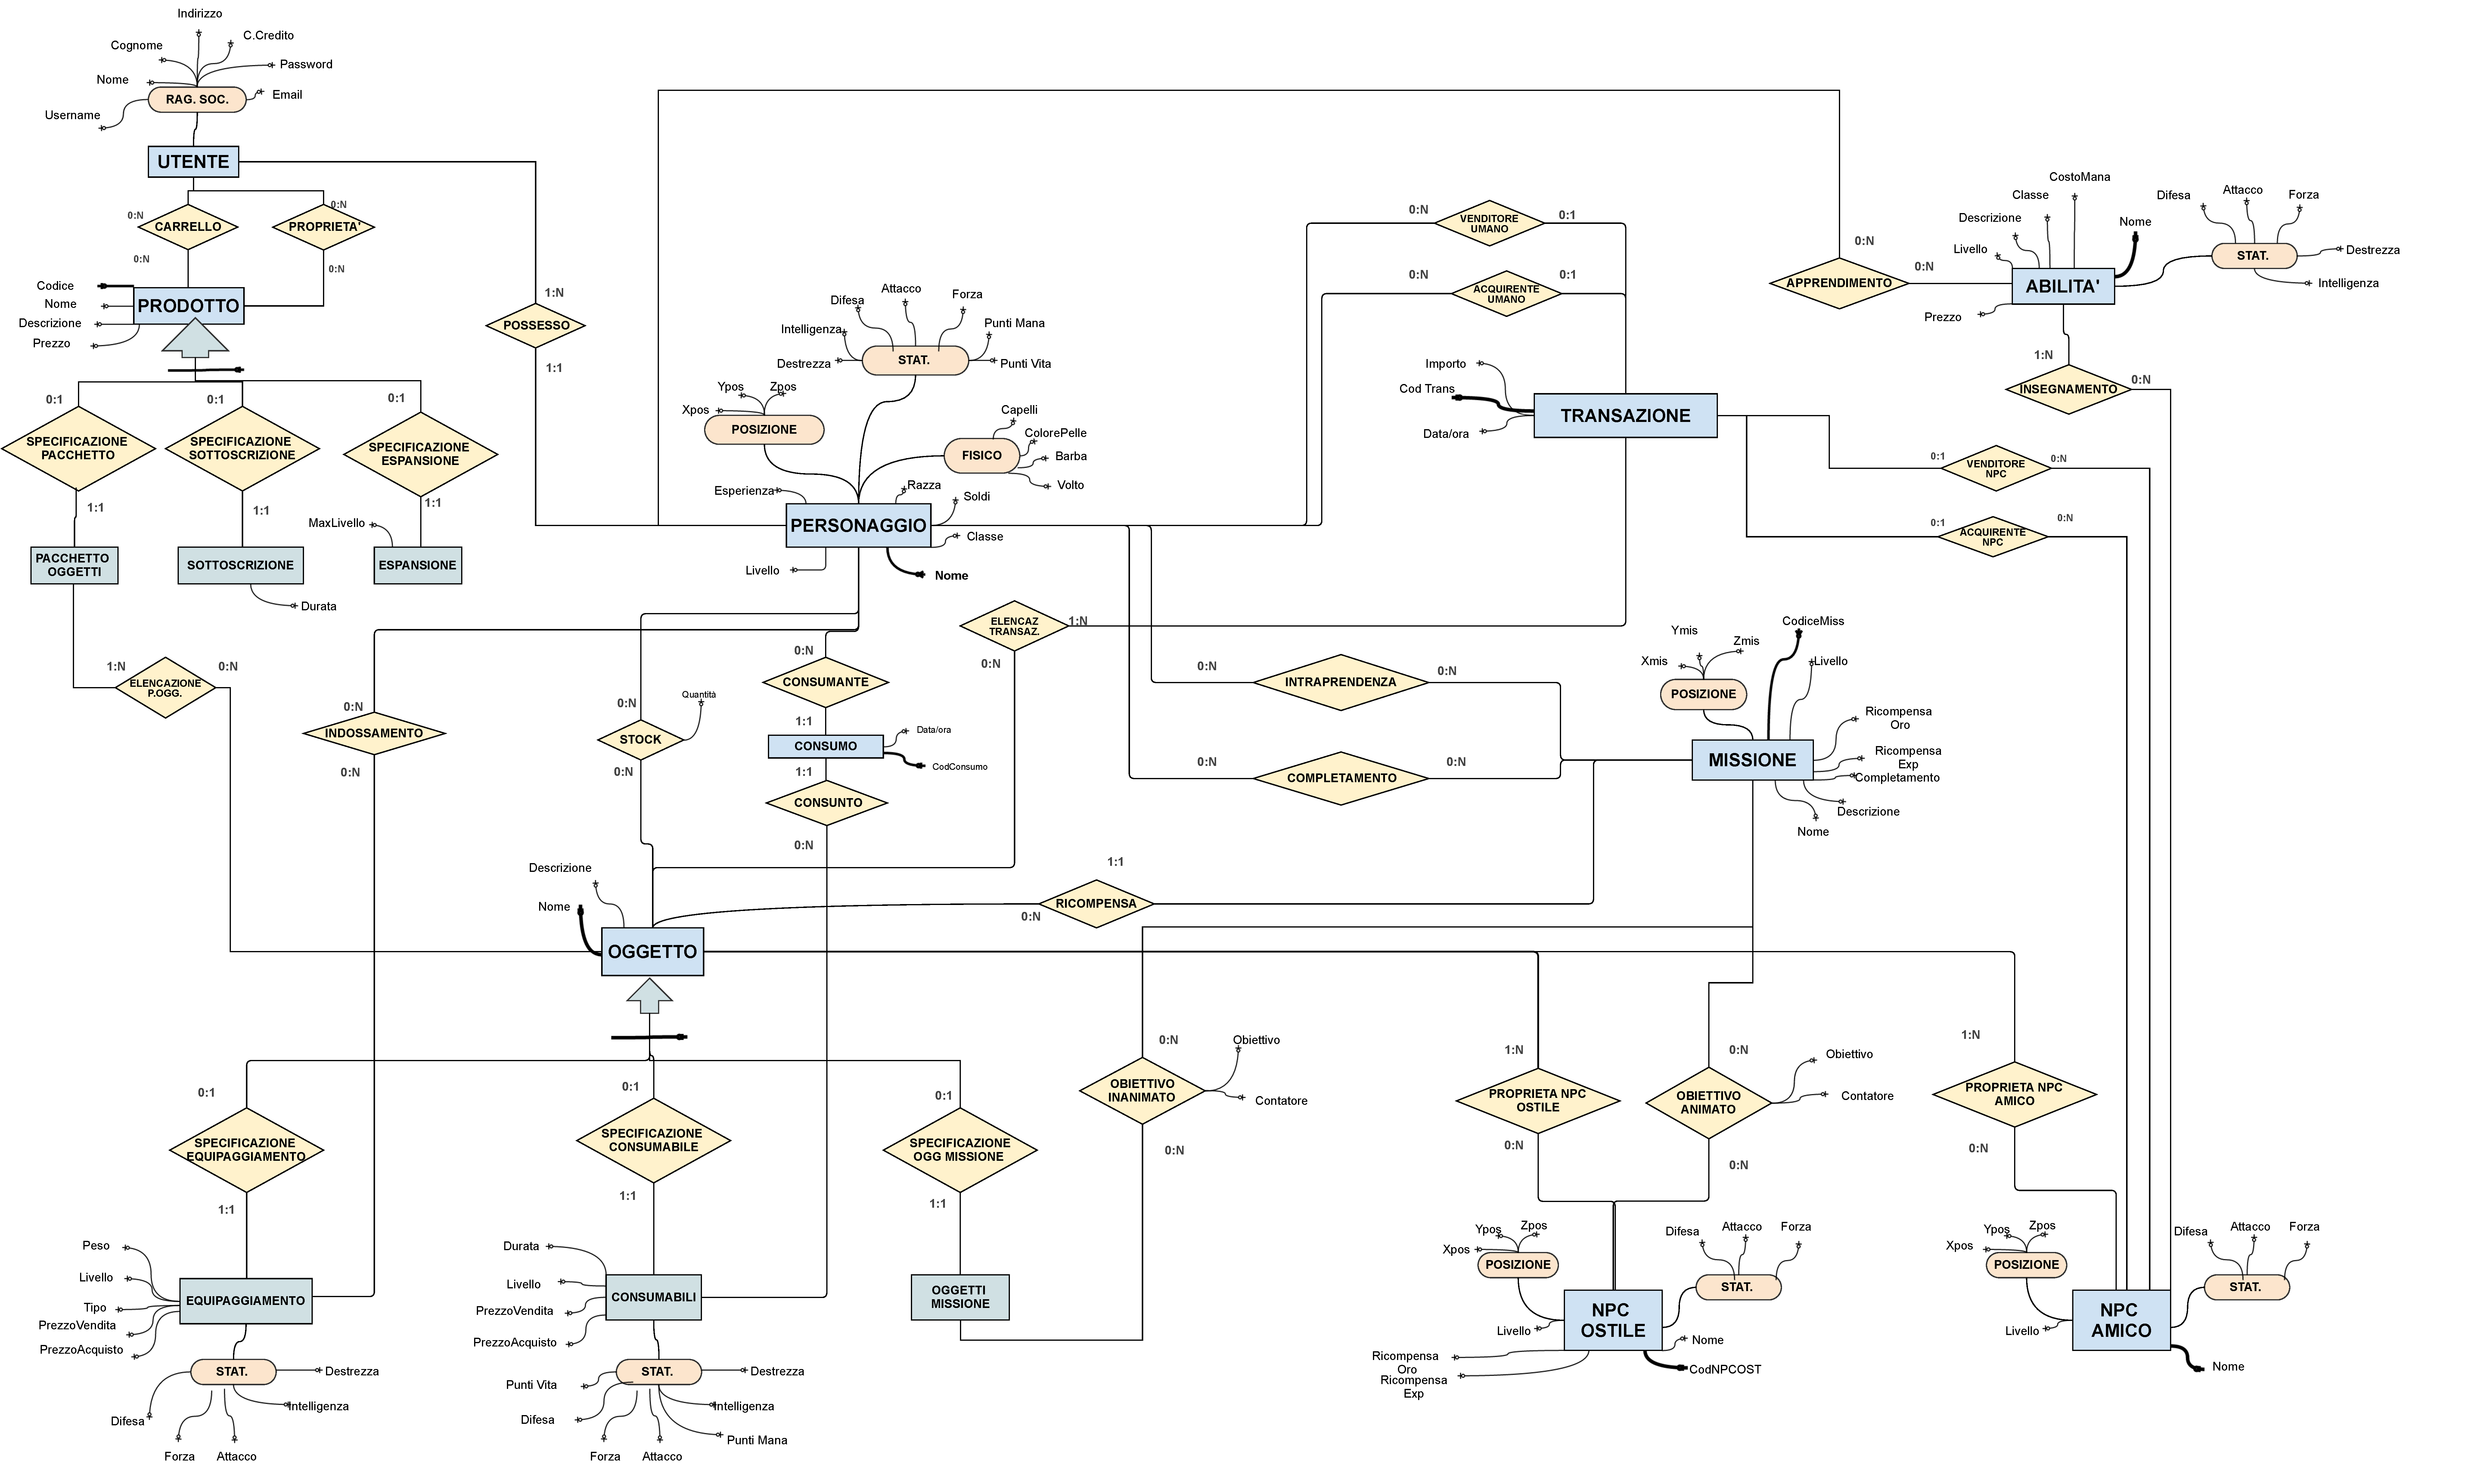
\includepdf[width=270mm, height=210mm, angle=90, keepaspectratio]{./pdf/ristrutturatosenzacarta.pdf}
%
% \end{landscape}


\newpage
\subsubsection{Eliminazione degli Attributi Multivalore}

Abbiamo individuato un solo attributo multivalore, l'attributo Telefono nelle entità Privato, Pubblica Amministrazione e Fornitore, in quanto abbiamo ritenuto che sia possibile che una di queste entità abbia più numeri di telefono associati.
\newline
Relativamente alle relazioni qui sopra citate abbiamo eseguito la ristrutturazione seguente:
\newline\newline

\noindent\makebox[\textwidth]{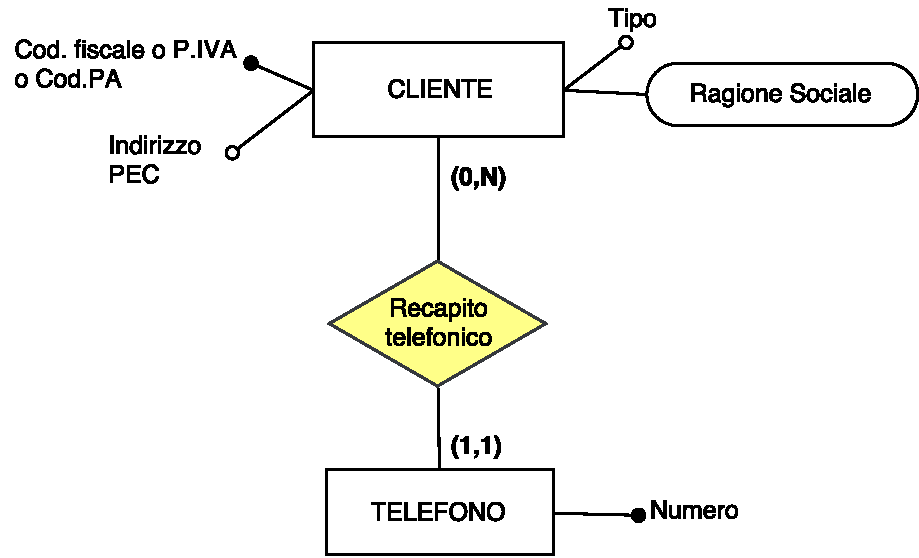
\includegraphics[width=0.7\linewidth]{./immagini/recapito_telefonico.pdf}}
\newline\newline
Tale ristrutturazione, relativa all'entità Pubblica Amministrazione, è analoga a Privato e Fornitore, perciò non vengono riportate le modifiche a tali entità.
